\section{In-beam Testing}
\subsection{Beam Time}
\subsubsection{2014 Test}
The beam tests for the EMMA PGAC took place from \longusdate\formatdate{25}{4}{2014} to \longusdate\formatdate{28}{4}{2014} with a total of 35.1\,hours of beam on target.  Data runs were recorded during the day, starting %at 12:53
 on \longusdate\formatdate{26}{4}{2014}. The tests used a beam of $^{16}$O at an energy of 1.103\,MeV$/u$ in a 3+ charge state.  A a 251\,$\mu$g/cm$^2$ gold target was used for the duration of the experiment.  The target is shown in Fig.~\ref{target}.  The target wheel was suspended from the lid of the scattering chamber.  The target being used was in the lower position.  After the experiment, the target appeared to have a burn mark on it.  The PGAC was installed on the HEBT beam line in the ISAC-I experimental hall as shown in Fig.~\ref{schematic}.

\begin{figure}%
\centering
\hspace{\fill}
\includegraphics[width=0.32\columnwidth,height=0.21\textheight,keepaspectratio]{IMG_3221dcR}\hspace{\fill}
\includegraphics[width=0.66\columnwidth,height=0.21\textheight,keepaspectratio]{IMG_3223_21}\hspace{\fill}
\caption{The 251\,$\mu$g/cm$^2$ gold target foil used for the duration of the experiment.  (Left) The target foil as seen by the beam.  (Right) The target foil, viewed downstream, as mounted on the target wheel.  Photos by A.\ Rojas.}%
\label{target}%
\end{figure}
Point of information: The incident beam energy of 1.103\,MeV$/u$ corresponds to a beam particle velocity of 14.58\,mm/ns.  After passing through the gold foil and the 2\,$\mu$m Mylar foil, the energy of the $^{16}$O beam particles is approximately 0.90\,MeV$/u$; corresponding to a velocity of 13.2\,mm/ns.  At this velocity, the transit time of the beam particles between the anodes is approximately 2.8\,ns.

\subsubsection{2015 Test}
The second in-beam test of the PGAC detector took place from \longusdate\formatdate{21}{4}{2015} to \longusdate\formatdate{23}{4}{2015}. A beam of $^{22}$Ne in the $4^+$ charge state was delivered with a nominal beam intensity of 8.5--22.4\,enA (2.1--5.6\,pnA) as measured on \texttt{HEBT:FC14}. A collimator was installed on the target wheel, however the target wheel adjustment mechanism did not have sufficient reproducibility. Therefore,  the 251\,$\mu$g/cm$^2$ gold foil used in the previous test was aligned to the beam axis using a theodolite and left in place for the duration of the experiment. The beam current was then monitored on \texttt{HEBT:FC19} at the end of the beam line. Note: the gold foil was accidentally destoyed during venting.


\subsection{Detector Configuration}
\begin{figure}
\centering
\hspace{\fill}
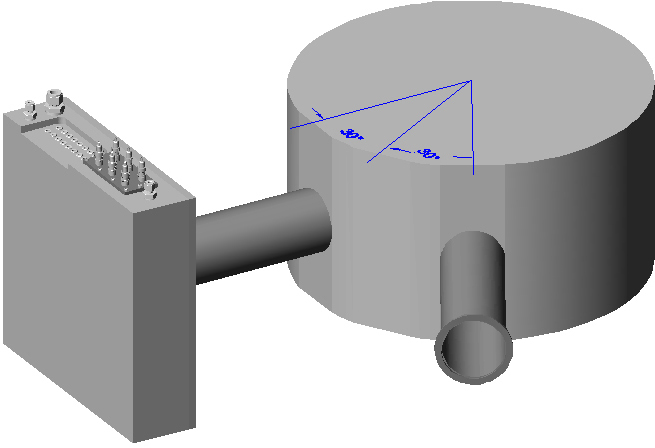
\includegraphics[width=0.48\textwidth,keepaspectratio]{HEBT_Scat_Chamber_3D_trim}\hspace{\fill}
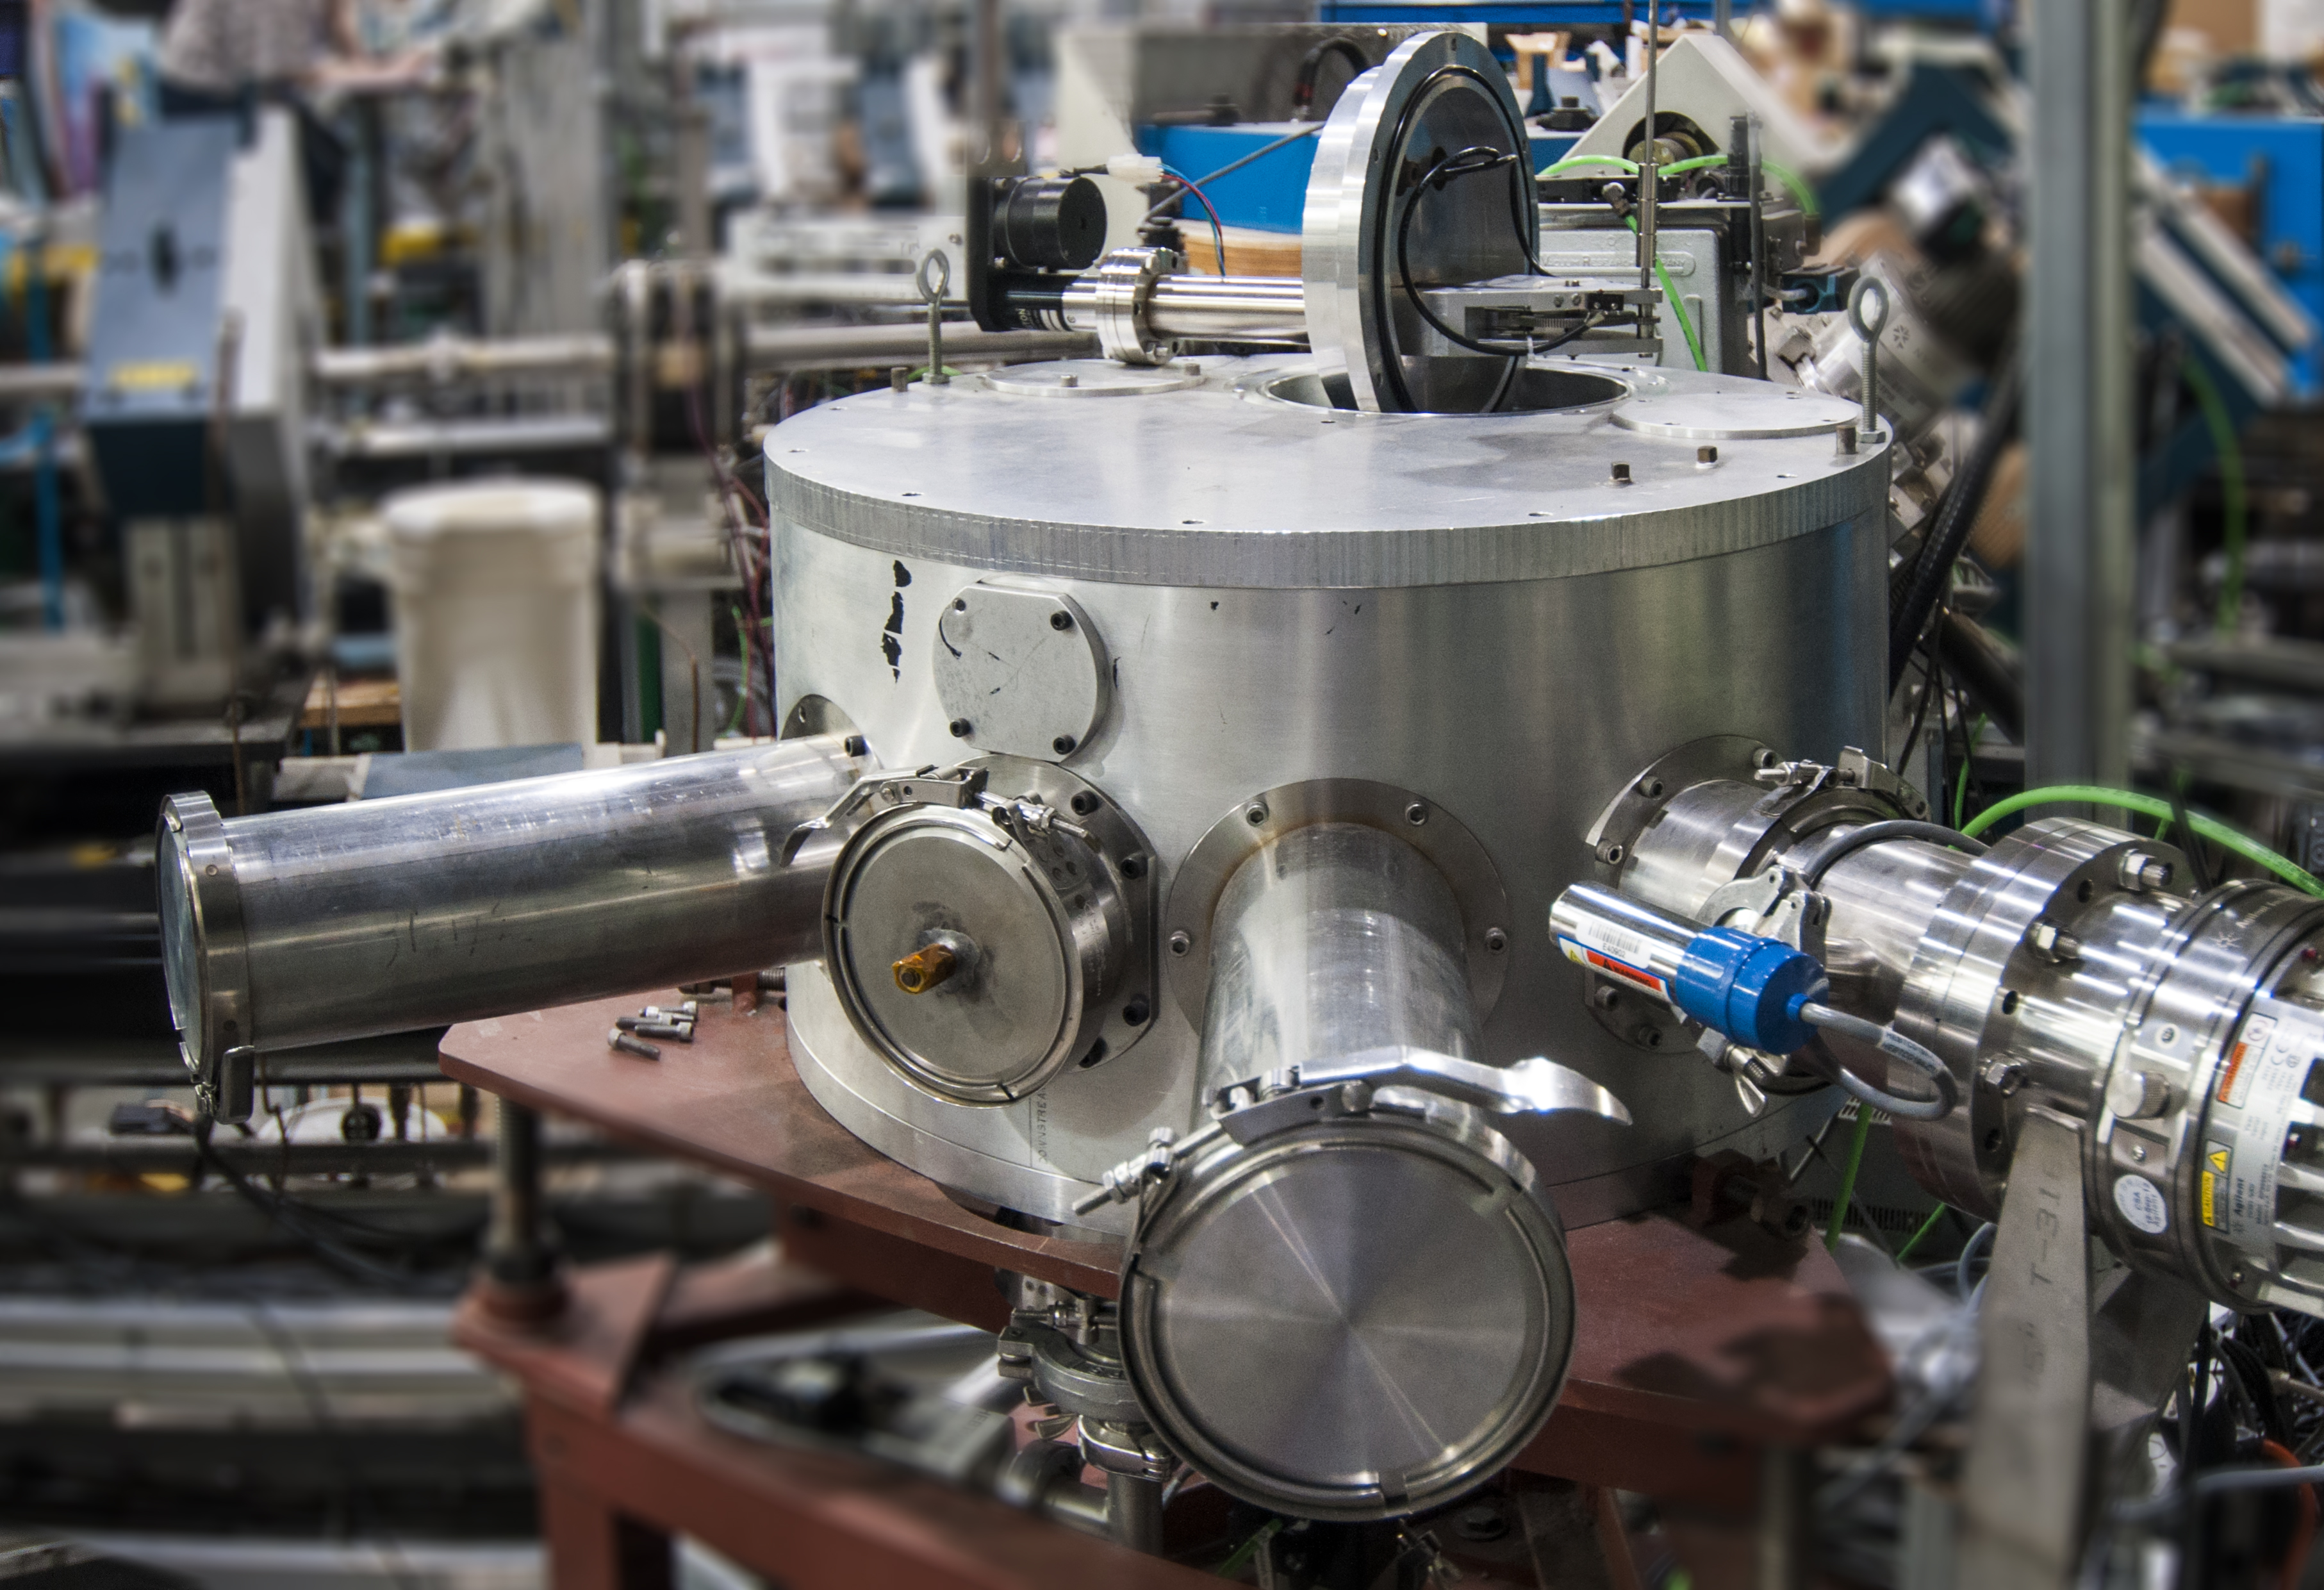
\includegraphics[width=0.48\textwidth, keepaspectratio]{DSC_0004} \hspace{\fill}
\caption{(Left) Schematic diagram of the experimental setup showing a view from downstream of the HEBT beam line.  The beam enters the 0$^\circ$ scattering chamber from the top of the figure.  The beam will bombard a target foil at the center of the chamber and scattering into the PGAC box, mounted at 30$^\circ$ relative to the beam line.  The length of the beam pipe connecting the PGAC box to the scattering chamber is such that 60\% of the active area of the PGAC will be illuminated.  (Right) A photograph of the 0$^\circ$ scattering chamber before PGAC box installation.}
\label{schematic}
\end{figure}
\subsubsection{Settings}
\paragraph{ }The PGAC was tested at four different pressures of %filled with
 isobutane---% 
 %at a pressures of 
 2, 3, 4 and 6\,Torr---%at various points
 during the experiment. The 12.6\,L internal gas volume of the PGAC box was separated from the vacuum of the 50\,L scattering chamber by a 2\,$\mu$m thick Mylar window. The maximum stable voltage was selected for each run, depending on the beam current and the gas pressure. The cathode voltage was varied from $-74$\,V to $-90$\,V and the anode voltage was varied from $+375$\,V to $+490$\,V.  The higher potential differences generally correspond to the higher pressures and the lower potential differences generally correspond to the lower pressures.
 \paragraph{2015 Test} The optimal voltage settings from the first test were used for the second test. The detectors were tested at three different pressures: 2, 3, and 4\,Torr. Low-rate tests at $10\times$ attenuation were  performed on the second and third days. A high-rate test with $17.7\times$ more beam current was also performed on the third day.
\subsubsection{Geometry}
The PGAC box was mounted to the scattering chamber at the end of the HEBT beam line at an angle of 30$^\circ$ relative to the beam line.  Fig.~\ref{schematic} includes a diagram of the experimental setup and a photograph of the scattering chamber. The PGAC was connected to the scattering chamber by a short beam pipe.  The length of the pipe was such that the plane of the %active area
anode of the first PGAC was 682.9\,mm from the target, as shown in Fig.~\ref{rays}.  With the center of the detector located at $\theta_\textrm{lab}=30^\circ$ relative to the beam.  This central trajectory corresponds to $\theta_\textrm{cm}=32.33^\circ$.

\begin{figure}
\centering
\includegraphics[width=\textwidth,keepaspectratio]{EMMA_Test_Stack_Scat_Cham}
\caption{(zoomable online) Orientation of the PGAC box relative to the HEBT scattering chamber. The relative positions of the mask and shield features are listed in Tables~\ref{zpos}, \ref{xpos}, and \ref{ypos}.}
\label{rays}
\end{figure}

The beam pipe shown in Fig.~\ref{rays} defines the minimum scattering angle illuminating the detectors $\theta_\textrm{lab}=30-4.47^\circ=25.5^\circ$ or $\theta_\textrm{cm}=27.5^\circ$.
The maximum scattering angle for each detector is defined by the %angular 
location of the edge of the Kapton shields, the angular position of which varies slightly for each detector.  For detector 2, the maximum scattering angle is $\theta_\textrm{lab}=33.0^\circ$ ($\theta_\textrm{cm}=35.6^\circ$); 89.5\,mm illuminated in the $x$-direction. For detector 1, the maximum scattering angle is $\theta_\textrm{lab}=32.9^\circ$ ($\theta_\textrm{cm}=35.4^\circ$); 92.3\,mm illuminated.
Fig.~\ref{rays} shows that the position of the frame of the Mylar window is in the same angular position as the rearmost Kapton shield for detector one. The alignment of the window frame may also define the maximum scattering angle.
%Therefore, 
Each detector covers about $\Delta \theta_\textrm{lab}=7.4^\circ$, subtending about 10.5\,msr in the laboratory.  The details of these calculations are discussed in Section~\ref{cal_def}.
\subsubsection{Rate}
Given an ion drift time in the PGAC of about 2\,$\mu$s, the desired maximum count rate in the detector was 250\,kHz.
\paragraph{2014 Test}The original beam request assumed that the entire fiducial area of the detector would be illuminated.  Therefore, given the Rutherford scattering cross section of the $^{16}$O beam from the gold foil target, this count rate corresponded to a beam rate of $3.9 \times 10^{10}$\,pps or 6.2\,pnA. During the experiment, three different beam attenuator settings were used.  For most of the experiment, the beam attenuator was set to $10\times$ with an average beam current on-target of 5.05\,enA. Four data runs used the $120\times$ attenuator setting (0.61\,enA) to test the low-count-rate performance of the detector. One data run used the $1\times$ ``attenuator'' (34.0\,enA) to test the high-count-rate performance of the detector.
\paragraph{2015 Test}
The nominal beam current was different each day. The nominal beam current for the three days of the experiment were as follows: 8.8\,enA on the first day, Tuesday, April 21, 2015; 12.7\,enA on the seconday; and  21.3\,enA on the third day.

\subsubsection{Mask}
A different mask was used during each of the in-beam experiments. They are shown in Fig.~\ref{mask} and Fig.~\ref{mask2}. The original mask featured a grid of 5\,mm wide strips. This mask provided a left-right orientation for the $x$-position signals however, it was not suitable for assessing the position resolution of the detector.
A new mask was developed for the 2015 tests featuring a 4.0\,mm $\times$ 4.0\,mm grid of 0.5\,mm holes. This mask allowed for the assessment of the position resolution of the detectors and the linearity of the position.

\begin{figure}
\centering
\includegraphics[width=\textwidth, keepaspectratio]{EMMA_Beam_Test_Mask_with_Kapton_v6.pdf}
\caption{Schematic diagram of the stainless steel mask used during the April 2014 in-beam tests. Dimensions are given relative to the Kapton shield.  The circular opening in the mask was coaxially aligned with the beam pipe and thus the beam.  The relative positions of the mask and shield features are listed in Tables~\ref{xpos} and \ref{ypos}.}%
\label{mask}%
\end{figure}

\begin{figure}[t]
\centering
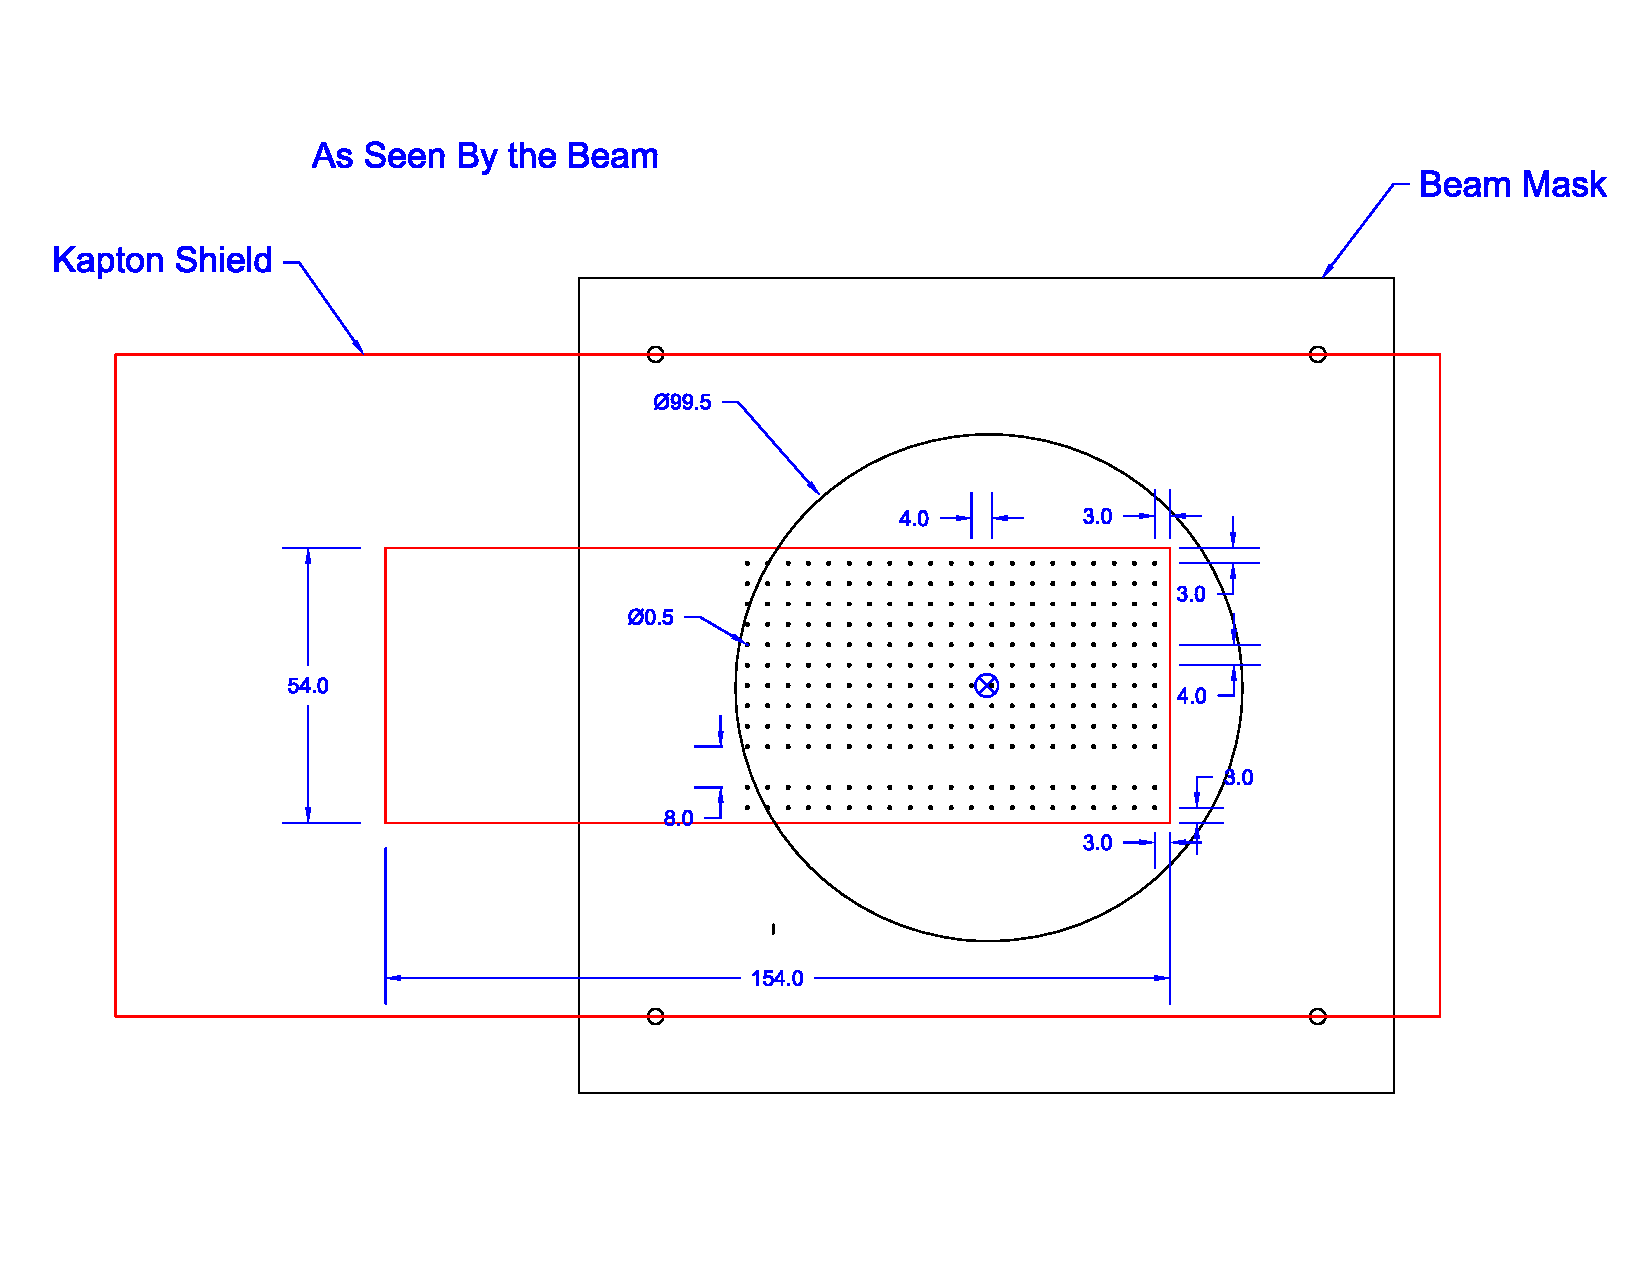
\includegraphics[width=\textwidth, keepaspectratio]{EMMA_Beam_Test_Hole_Mask_2}
\caption{Schematic diagram of the stainless steel mask used during the April 2015 in-beam tests. A 4\,mm lattice of holes was used. Dimensions are given relative to the Kapton shield.  The large circle indicates the diameter of the beam pipe.  The relative positions of the mask and shield features are listed in Table~\ref{xpos2}.
The position of the beam spot is the same as that given in Fig.~\ref{mask}.}%
\label{mask2}%
\end{figure}

\subsection{Electronics Configuration}
The electronics setup is illustrated schematically in Fig.~\ref{e-diagram}.
\begin{figure}[p]
\centering
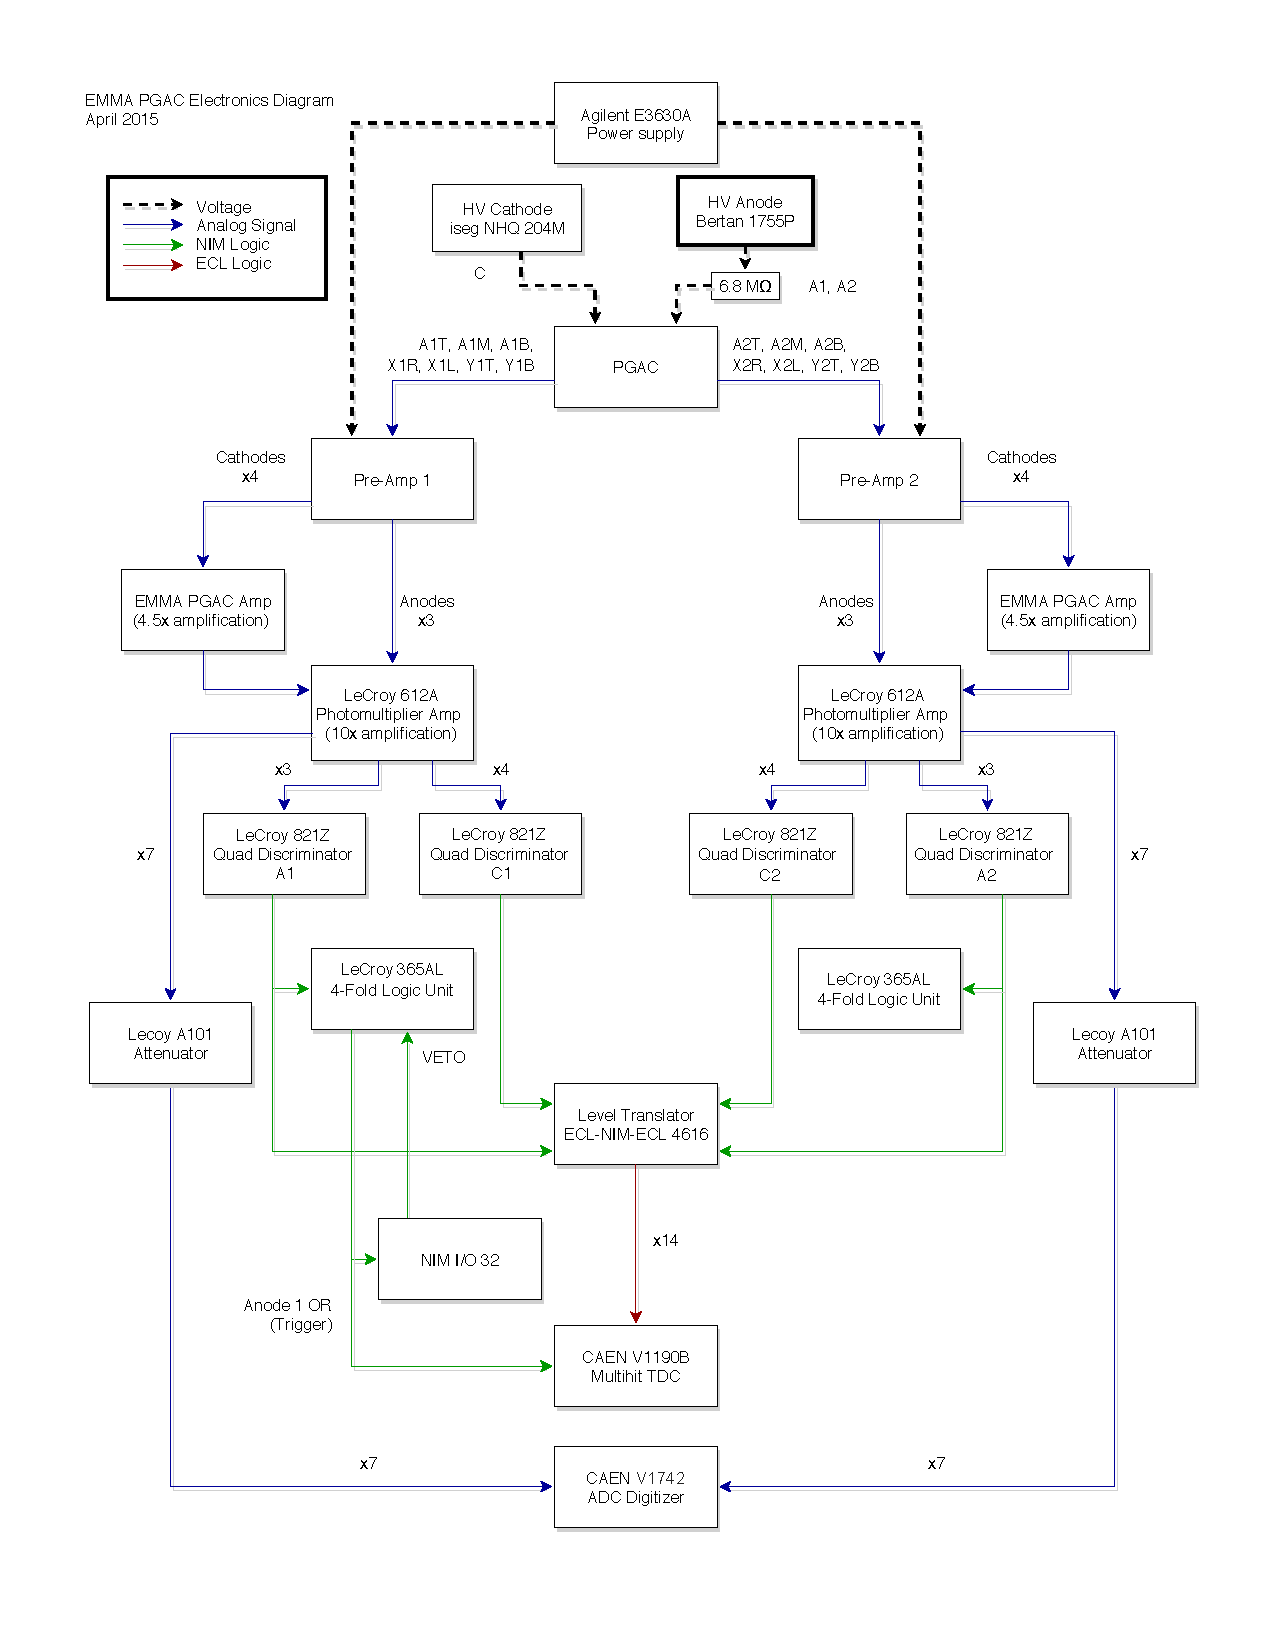
\includegraphics[width=\textwidth, keepaspectratio]{electronics_diagram}
\caption{Electronics diagram for the PGAC tests. Each signal is amplified and passed through a level discriminator to generate a logic signal. The logic signals are read in by the TDC. The logical OR of the anode signals us used to generate the acquisition trigger. A copy of each amplified signal is passed through an attenuator and read in by the waveform digitizer. Drawn by C.\ Ward and R.\ Baker-French.}%
\label{e-diagram}%
\end{figure}
The settings for the TDC, ADC, and pulser were set in MIDAS following the beginning of each run. These settings, in addition to the start and stop time for each run, were recorded in the file \texttt{midas.log} located in  the directory 
\verb|/home/emma/online/| on the LADD cluster. Currently the \texttt{midas.log} file is over 25\,MB in size due to large number of error messages. Removing these lines\footnote{Lines can be removed in emacs using the command \texttt{M-x delete-matching-lines} or \texttt{M-x delete-non-matching-lines}.} reduces the file size to less than 400\,kB.
%\begin{changemargin}{-1in}
%\pangram{100}  
%\end{changemargin}
\subsubsection{Amplifiers}
\label{amp-settings}
All seven signals from each PGAC detector were passed through pre-amplifiers mounted to the PGAC box.  These pre-amplifers were custom built by the Detector Group.  The pre-amp signals were then further amplified using linear fast timing amplifiers.  Two different amplifiers were used: custom-built amplifiers providing approximately 4.5$\times$ amplification and standard %LeCroy xxx 
NIM modules, which provide approximately 10$\times$ amplification. Initially, during the beginning of the data runs, the anode signals were un-amplified and the cathode signals were amplified only  with the the custom-built amplifiers.

The discriminators being used had a minimum threshold setting of 30\,mV and sufficiently low discrimination thresholds were not possible with this configuration. Starting with Run 437, an additional $10\times$ amplification step was added to all of the signals. The added amplification allowed the discriminator thresholds to be set appropriately low. The added amplification step allowed the ratio of the signal peak height to the discriminator threshold level to be reduced by an average factor of $6.5\times$ for the anodes, which produce the trigger. The various discriminator settings are shown in Table~\ref{amp_1_step}.
%
%\begin{figure}
%\centering
%%\includegraphics[width=\textwidth, keepaspectratio]{}
%\textit{<figure to follow>}
%\caption{Electronics diagram.}%
%\label{e-diagram}%
%\end{figure}
\renewcommand{\tabcolsep}{2pt}
\begin{table}[ht!]
\begin{changemargin}{-0em}
\centering  
\hspace{\fill}
\begin{tabular}{c.....}
\hline
\multicolumn{1}{c}{Signal} & \multicolumn{1}{c}{PA}& \multicolumn{1}{c}{Disc} & \multicolumn{1}{c}{Amp} & \multicolumn{1}{c}{Thresh} &\multicolumn{1}{c}{Ratio}\\
&\multicolumn{1}{c}{mV} & \multicolumn{1}{c}{mV}&& \multicolumn{1}{c}{mV} & \textrm{}  \\ \hline \hline
\texttt{A1B} & 112.3 & 112.3 & 1.00 & 30.10 & 0.268 \\
\texttt{A1M} & 120.2 & 120.2 & 1.00 & 30.10 & 0.250 \\
\texttt{A1T} & 122.8 & 122.8 & 1.00 & 30.20 & 0.246 \\
\texttt{A2B} & 135.5 & 135.5 & 1.00 & 60.70 & 0.448 \\
\texttt{A2M} & 124.5 & 124.5 & 1.00 & 30.00 & 0.241 \\
\texttt{A2T} & 130.2 & 130.2 & 1.00 & 29.90 & 0.230 \\
\texttt{X1L} & 37.2 & 179.8 & 4.83 & 30.00 & 0.167 \\
\texttt{X1R} & 34.6 & 157.7 & 4.56 & 30.00 & 0.190 \\
\texttt{Y1B} & 40.5 & 180.9 & 4.47 & 30.00 & 0.166 \\
\texttt{Y1T} & 37.1 & 167.6 & 4.52 & 30.20 & 0.180 \\
\texttt{X2L} & 39.9 & 172.3 & 4.32 & 30.20 & 0.175 \\
\texttt{X2R} & 38.8 & 178.0 & 4.59 & 30.00 & 0.169 \\
\texttt{Y2B} & 42.0 & 190.8 & 4.54 & 30.40 & 0.159 \\
\texttt{Y2T} & 43.2 & 191.6 & 4.44 & 30.00 & 0.157 \\
\hline 
\end{tabular}
\hspace{\fill} \begin{tabular}{c.....}
\hline
\multicolumn{1}{c}{Signal} & \multicolumn{1}{c}{PA}& \multicolumn{1}{c}{Disc} & \multicolumn{1}{c}{Amp} & \multicolumn{1}{c}{Thresh} &\multicolumn{1}{c}{Ratio}\\
&\multicolumn{1}{c}{mV} & \multicolumn{1}{c}{mV}&& \multicolumn{1}{c}{mV} & \textrm{}  \\ \hline \hline
\texttt{A1B} & 127.0 & 1100.0 & 8.66 & 55.00 & 0.050 \\
\texttt{A1M} & 123.0 & 1170.0 & 9.51 & 60.00 & 0.051 \\
\texttt{A1T} & 120.0 & 1130.0 & 9.42 & 65.00 & 0.058 \\
\texttt{A2B} & 137.0 & 1510.0 & 11.02 & 55.00 & 0.036 \\
\texttt{A2M} & 126.0 & 1420.0 & 11.27 & 56.00 & 0.039 \\
\texttt{A2T} & 131.0 & 1520.0 & 11.60 & 57.00 & 0.038 \\
\texttt{X1L} & 36.0 & 1670.0 & 46.39 & 58.00 & 0.035 \\
\texttt{X1R} & 34.0 & 1650.0 & 48.53 & 200.00 & 0.121 \\
\texttt{Y1B} & 41.0 & 1850.0 & 45.12 & 210.00 & 0.114 \\
\texttt{Y1T} & 39.0 & 1740.0 & 44.62 & 200.00 & 0.115 \\
\texttt{X2L} & 40.0 & 1850.0 & 46.25 & 200.00 & 0.108 \\
\texttt{X2R} & 40.0 & 1800.0 & 45.00 & 200.00 & 0.111 \\
\texttt{Y2B} & 44.0 & 1960.0 & 44.55 & 200.00 & 0.102 \\
\texttt{Y2T} & 43.0 & 1910.0 & 44.42 & 200.00 & 0.105 \\
\hline 
\end{tabular}
\hspace{\fill}
\caption{Discriminator values before and after the inclusion of an extra $10\times$ amplification. The signal level at the output of the preamplifier (PA) and at the input of the discriminator (Disc) is given. The ratio of these two values gives the amount of amplification applied to the signal (Amp). The discriminator threshold (Thresh) is also given. The minimum discriminator threshold was 30\,mV. Finally, the ratio of the discriminator threshold to the discriminator input signal is given. For both amplification settings, the detector had the following settings $P=3$\,Torr, $V_\textrm{a}=410$\,V, $V_\textrm{c}=-75$\,V, $\Delta V=485$\,V. }
\label{amp_1_step}
\end{changemargin}
\end{table}
\renewcommand{\tabcolsep}{6pt}%\the\tabcolsep

\subsubsection{TDC}The detector signals were read into the acquisition system using two different methods.  The first method used a time-to-digital converter (TDC), specifically a CAEN V1190B-2eSST 64 Channel Multihit TDC module.  The TDC has a full range of 4,0$96 \times 10$ channels and was configured for 200\,ps per channel. The TDC measures the arrival time of logic pulses relative to a trigger pulse.   The amplified signals from the PGAC were entered into leading-edge discriminators to produce the logic signals required by the TDC.  The logical OR of the anode signals of detector 2 (the detector facing the beam) was used to generate the trigger.
\begin{table}%

\begin{minipage}{\textwidth}
\begin{center}
  

%
%
\begin{tabular}{rrr|rrcc|cc}
%\multicolumn{1}{c}{Plane} & \multicolumn{1}{c}{$z$-position} \\ 
\hline
%\multicolumn{1}{c}{TDC\footnote{April 2014}} & \multicolumn{1}{c}{TDC\footnote{April 2015}} &

\multicolumn{2}{c}{TDC} & %\multicolumn{1}{c}{TDC} &

\multicolumn{1}{c}{ADC} &\multicolumn{1}{|c}{Label}& \multicolumn{1}{c}{Pair} & Position & Side & Branch & Leaf \\
\cline{1-2} 
\multicolumn{1}{c}{2014} & \multicolumn{1}{c}{2015} & \multicolumn{1}{c}{}\\
\hline \hline
 0 &  0 &  0 &\texttt{A1B} & 0 & bottom & ---&PGAC1&ab\\
 1 &  1 &  1 &\texttt{A1M} & 1 & middle & ---&PGAC1&am\\
 2 &  2 &  2 &\texttt{A1T} & 2 & top & ---&PGAC1&at\\
 3 &  3 &  3 &\texttt{A2B} & 0 & bottom & ---&PGAC2&ab\\
 4 &  4 &  4 &\texttt{A2M} & 1 & middle & ---&PGAC2&am\\
 5 &  5 &  5 &\texttt{A2T} & 2 & top & ---&PGAC2&at\\ \hline 
 6 &  {\color{red}9} &  8 &\texttt{X1L} & 3 & right & far&PGAC1&xf\\
 7 &  {\color{red}8} &  9 &\texttt{X1R} & 3 & left & near&PGAC1&xn\\
 8 &  {\color{red}7} & 10 &\texttt{Y1B} & 4 & bottom & near&PGAC1&yn\\
 9 &  {\color{red}6} & 11 &\texttt{Y1T} & 4 & top & far&PGAC1&yf\\
10 & 10 & 12 &\texttt{X2L} & 5 & right & far&PGAC2&xf\\
11 & 11 & 13 &\texttt{X2R} & 5 & left & near&PGAC2&xn\\
12 & 12 & 14 &\texttt{Y2B} & 6 & bottom & near&PGAC2&yn\\
13 & 13 & 15 &\texttt{Y2T} & 6 & left & far&PGAC2&yf\\
 \hline 
\end{tabular}
\end{center}
\end{minipage}

\caption{Input signals to the TDC and ADC.  Note that in the April 2015 tests, the position signals for detector 1 were plugged in backwards. Note also that the signals input to the ADC are split into two groups: signal inputs 0--5 and inputs 8--15. The 14 signals formed 7 pairs.  The position are given as seen by the beam.  For each position, signals are ``near'' or ``far'' relative to the bottom left corner of the fiducial area of the detector. The branch and leaf names for tree sorting are also given.}
\label{TDC_signals}
%
\end{table}

The detector signals were connected to the TDC in the order shown in Table~\ref{TDC_signals}. Ideally, all 14 signals (7 from each detector) would have been read into the TDC.  In this manner, the signal from each segment of the anode is read in independently.  However, only the logical OR of the anode signal was read into the TDC.  Therefore, each detector had 5 signals associated with it.  The ORs of the anode signals for each detector were read into the channel corresponding to the A$n$M signal.

\subsubsection{Digitizer}Copies of the amplified detector signals were also fed into a waveform digitizer, specifically a CAEN V1742 32+2 Channel 12-bit 5\,GS/s Switched Capacitor Digitizer module. 
The V1742 is based on two DRS4 (%\footnote{DRS4 is an abbreviation of 
Domino Ring Sampling, revision 4) %.}
 chips, each with $16+1$ channels.  %Each channel has a fixed jitter constant that needs to be corrected for during calibration.
Each of the 16+1 channel groups have their own trigger and are further divided into two input signal groups. % These groups  
%The inputs of the V1742 are divided into two different groups, corresponding to signals 0--7 and 8--15.
Each of the two input groups has an independent timing correction. Table~\ref{TDC_signals} shows that the anodes of both detectors were input into the first group and the cathodes were input into the second group.

%\marnote{check}
Of the 69 total data runs, 47 of them had the digitizer enabled.
 The digitizer was operated at 1.0, 2.5, and 5.0\,GS/s.  These sample rates correspond to timing resolutions of 1.00\,ns, 400\,ps, and 200\,ps, respectively.
 Since the V1742 is an analogue digitizer, the memory buffer has a fixed size of 1024 cells. The different sample rates correspond to acquisition windows of 1.024\,$\mu$s, 409.6\,ns, and 204.8\,ns, respectively.
 During most of the runs the digitizer was set to 1.0\,GS/s. For 7 data runs the digitizer was set to 2.5\,GS/s and for 10 data runs it was set to 5.0\,GS/s.  The digitizer settings were written to memory \textit{after} the start of each run and could not be changed during the run. Care must be taken when parsing MIDAS log file to ensure that the digitizer status  is properly associated with the correct run number.
 %written \textit{after} the start of the run is the setting for that run.
 
 The analog input dynamic range of the TCDC is 1\,V peak-to-peak.  Therefore, depending on the detector bias and the amplification, the amplified detector signals needed to be attenuated in order to fit within the 1\,V range of the digitizer.  An array of independently adjustable 50\,$\Omega$ attenuators was used to provide the minimum attenuation required to keep the peak-to-peak signal amplitude under 1\,V.  Typical values of attenuation was 0.5$\times$.
	
